\chapter{Cooperation}\label{ch:cooperation}
\begin{chapter_outline}

This chapter introduces the main concepts of learning to cooperate with multi-agent reinforcement learning.
While both chapters \ref{ch:qvmix} and \ref{ch:impmarl} present our contributions in this field, this chapter covers the related works in the literature.
After a small introduction in Section \ref{sec:ch3_intro}, we define the decentralised POMDP, an adaptation of the stochastic game to the cooperative setting in Section \ref{sec:ch3_decpomdp}.
Once defined, examples of such environments are provided in Section \ref{sec:ch3_env}.
We then present methods designed to solve such environments, respectively value-based methods in Section \ref{sec:ch3_value} and policy-based methods in Section \ref{sec:ch3_policy}.
Finally, we conclude with a related work discussion in Section \ref{sec:ch3_rel_work} presenting methods and framework from the literature that goes beyond the content of this manuscript.

\end{chapter_outline}


\section{Introduction}
\label{sec:ch3_intro}
As introduced in Part \ref{part:background}, cooperation is the multi-agent setting of agents sharing a common goal.
This manuscript considers the decentralised POMDP (Dec-POMDP), a framework where all agents receive the same reward.
Its definition, provided in Section \ref{sec:ch3_decpomdp}, can be easily derived from the partially observable stochastic game one because only the reward function changes to provide the same reward to all agents.
Such a framework is also called common reward games, e.g. in \cite{marl-book}.

\todo{However, others settings..}

Nevertheless, when it comes to cooperation in a multi-agent system, one notion to discuss is whether the action selection and the training of agents are centralised or decentralised.
The difference lies in the information shared or not by agents.
This is referred to, in \citep{marl-book}, as the modes of execution and training.
This manuscript considers three combinations: centralised training and execution, decentralised training and execution, and centralised training with decentralised execution.

Since all agents share a common goal, we could centrally select all actions, sharing common knowledge.
This is the centralised mode, where agents are commonly trained with single-agent reinforcement learning methods.
For example, controlling a robotic hand composed of several actuators can be done with a single agent controlling every one of its actuators.
However, as presented in Section \ref{sec:ch2_partial_observability}, all agents may not access the same information or may perceive only a part of the state of the environment.
It would then be impossible, except in a simulated environment, to consider that agents can easily select actions in a centralised mode, with information not available to every one of them.

On the contrary, the decentralised execution mode is the one that considers that each agent has only access to a subset of the information, the one it perceives, and uses it to select its action.
The corresponding decentralised training mode is when we train these agents based only on this perceived information.
We thus refer to the decentralised mode when training agents independently with single-agent reinforcement learning, assuming they are alone in the environment.

Finally, unifying the two former modes, the third one is the centralised training with decentralised execution (CTDE).
It allows decentralised execution, with each agent selecting actions based on their perceptions but exploiting more information during training.
Indeed, RL agents are usually trained in a simulator, having access to every piece of information.
Therefore, using the state of the environment or the actions made by other agents is possible.
Part \ref{part:coop} of this manuscript focuses on methods that exploit the CTDE mode to solve cooperative tasks.
This Chapter presents Dec-POMDP environments and CTDE methods issued from the literature. 
In contrast, both next Chapters present our contributions: a new CTDE method in Chapter \ref{ch:qvmix} and a new real-world environment in Chapter \ref{ch:impmarl}.

\section{Decentralised partially observable Markov decision process}
\label{sec:ch3_decpomdp}
The definition of the decentralised partially observable Markov decision process (Dec-POMDP) \citep{DecPomdp} can be derived from the stochastic game definition presented in Section \ref{sec:ch2_stochastic_Game}.
It is substantially the same, but the reward function maps only to a single real, a reward common to all agents.

We hereafter define the Dec-POMDP by a tuple $[\mathcal{S}, \mathcal{Z}, \mathcal{U}, n, O, R, P, \gamma]$, where $n$ agents $a_i$, $i \in \mathcal{A} \equiv \{1,..,n\}$, simultaneously choose an action at every time step $t$.
The state of the environment is $s_t \in \mathcal{S}$ where $\mathcal{S}$ is the set of states.
The observation function $O: \mathcal{S} \times \mathcal{A} \rightarrow \mathcal{Z}$ maps the state to an observation $o_t^{a} \in \mathcal{Z}$ perceived by agent $a$ at time $t$, where $\mathcal{Z}$ is the observation space.
Each agent $a_i$ selects an action $u_t^{a_i} \in \mathcal{U}^{a_i}$, and the joint action space is $\mathcal{U}$.
After the joint action $\boldsymbol{u_t} \in \mathcal{U}$ is executed, the transition function determines the new state with probability $P(s_{t+1}|s_t, \boldsymbol{u_t}): \mathcal{S} \times \mathcal{S} \times\mathcal{U} \rightarrow  [0,1] $, and $r_t=R(s_{t+1}, s_t, \boldsymbol {u_t}): \mathcal{S} \times \mathcal{S} \times \mathcal{U} \rightarrow \mathbb{R}$ is the team reward obtained by all agents.

An agent's policy is a function $\pi^{a}(u_t^{a}|\tau_t^{a},o_t^{a}): (\mathcal{Z} \times \mathcal{U}^a)^t \rightarrow [0,1]$, which maps its history $\tau_t^{a} \in (\mathcal{Z} \times \mathcal{U}_a)^{t-1}$ and its observation $o_t^{a}$ to the probability of taking action $u_t^{a}$. 
The joint policy, or team policy, is denoted by $\boldsymbol{\pi}=(\pi^1,..,\pi^n)$.
The cumulative discounted reward obtained from time step $t$ over the next $T$ time steps is defined by $G_{t} = \sum_{k=0}^{T-1} \gamma^k r_{t+k}$ and $\gamma \in [0, 1)$ is the discount factor.
The goal of agents is to find the optimal joint policy that maximises the expected $G_t$ during the entire episode: $\boldsymbol{\pi^{*}} =\argmax_{\boldsymbol{\pi}} \mathbb{E}[G_0|\boldsymbol{\pi}]$.
Again, we emphasise that this expected sum depends on the joint policy.

\todo{oliehoek: individually observable and jointly observable}

\todo{check concordance with notation of stochastic game}

\todo{check environment vs suite of environments}

\todo{Challenges in Dec-POMDP}

\section{Environments}
\label{sec:ch3_env}
Before diving into the details of CTDE methods, we provide an overview of the existing suites of environments from the literature.
We then describe the StarCraft multi-agent challenge (SMAC), perhaps one of the most studied environment suites in the community, but also used in our experiments in Chapter \ref{ch:qvmix}.
Moreover, Chapter \ref{ch:impmarl} is dedicated to a new suite of environments, and we leave its description there.

The multi-agent particle environments (MPE) \citep{lowe2017multi} is a popular suite in the MARL community with cooperative scenarios.
In MPE, particles move in a 2D grid with continuous action and state spaces.
This suite comes with all types of multi-agent settings: competition, cooperation, with and without competition.
A second environment with continual action space is MaMuJoCo \citep{peng2021facmac}.
MuJoCo \citep{todorov2012mujoco} stands for multi-joint dynamics with contact.
It is a famous physics-based simulator to learn to control, for example, a humanoid to run.
MaMuJoCo essentially factorises the decisions of MuJoCo by decentralising the decision.
It is an example of a SARL environment extended to MARL.
Other cooperative environments based on game simulators include the Hanabi Challenge \citep{Bard_2020}, a "cooperative solitaire" between two and five players, and Google Research Football \citep{kurach2020google}, a football game simulator.

Cooperative MARL methods are mostly benchmarked on these games and simulators but also on real-world applications.
City flow \citep{zhang2019cityflow} are traffic control environments where agents control traffic lights.
In Flatland \citep{mohanty2020flatland}, agents control trains to solve a scheduling problem, avoiding collisions.
The multi-robot warehouse \citep{papoudakis2021benchmarking, christianos2020shared} simulates warehouse agents needing to deliver requested goods.
Multi-Agent Tracking Environment (MATE) \citep{NEURIPS2022_b2a1c152} is a target coverage control problem where cameras are controlled to detect all targets where a mixed cooperative-competitive game can be made by controlling the targets.
Finally, there exist more examples of cooperative MARL applications.
Many can be found in the book of \cite{marl-book} or the review on cooperative MARL done by \cite{oroojlooy2022review}, such as autonomous driving, resource allocation, stock market,...

\subsection{StarCraft multi-agent challenge}
The StarCraft multi-agent challenge (SMAC) \citep{samvelyan2019starcraft} and its improved version SMACv2 \citep{ellis2022smacv2} are probably the most studied environments when comparing CTDE methods.
SMAC is based on the StarCraft II Learning Environment \citep{vinyals2017starcraft}, an RL environment to play StarCraft II (SC2).
StarCraft is a strategy video game where players compete by managing units, gathering resources, building an army and defeating opponents.
In such games, micro-management refers to unit management, unlike macro-management, which involves resource management.
Unlike playing StraCraft like AlphaStar \citep{vinyals2019grandmaster}, SMAC is a suite of micro-management challenges where each game unit is an agent.
Many scenarios exist in SMAC, but all involve training a team to achieve a common goal.
Still, this common goal is mostly to defeat an adversarial team controlled by the game's deterministic and stationary policy built-in AI.
In Figure \ref{fig:ch3_smac}, we present the initial configurations of two scenarios, also called maps, where two teams face each other.
Note that in Chapter \ref{ch:2teams}, we modify SMAC to train both competing teams.

\begin{figure}
     \centering
     \begin{subfigure}[b]{0.5\textwidth}
         \centering
         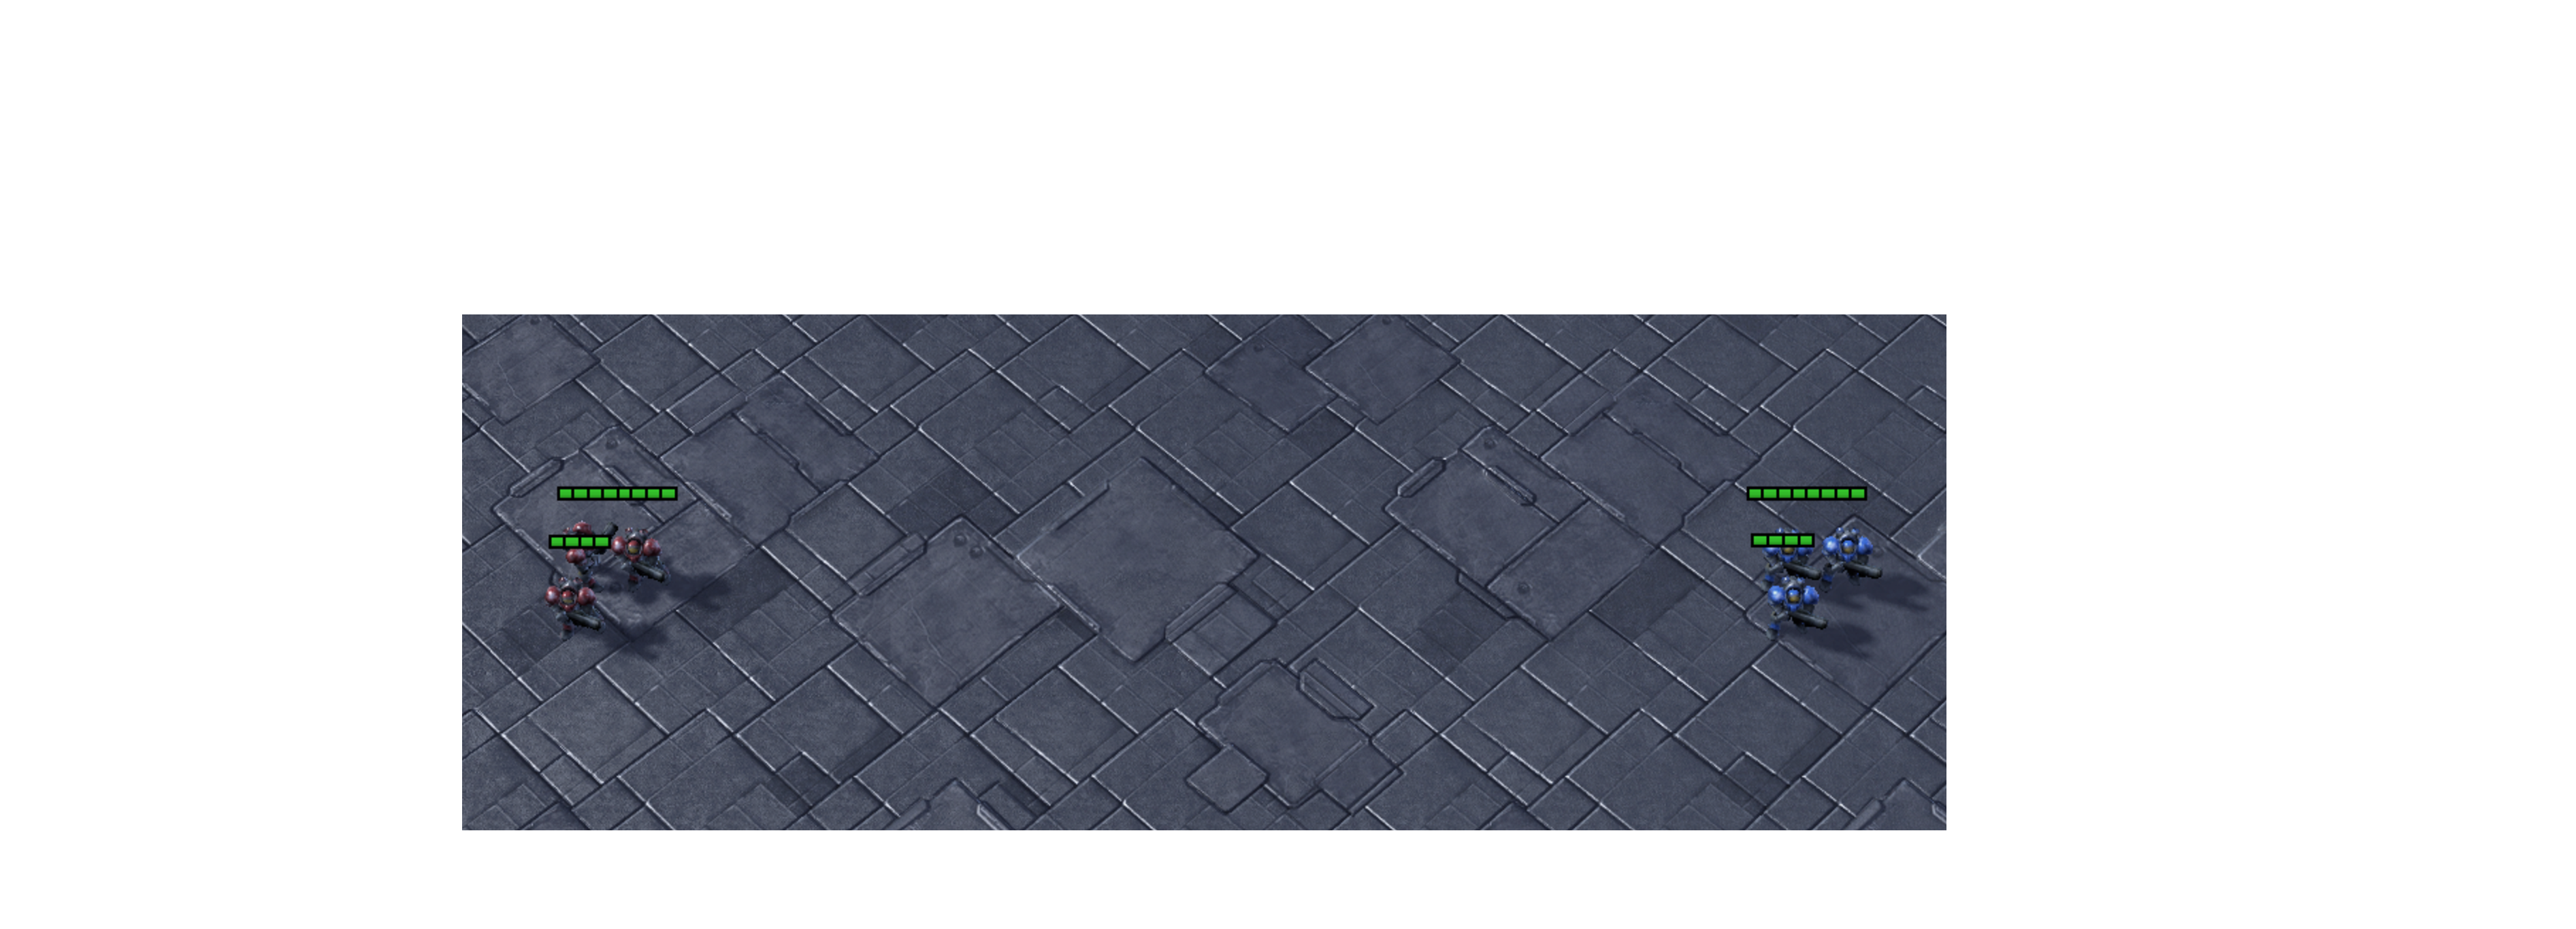
\includegraphics[height=2.3cm]{tex_thesis/figures/ch3/3m_screen.pdf}
         \caption{3m}
         \label{fig:ch3_3m}
     \end{subfigure}%
     \begin{subfigure}[b]{0.5\textwidth}
         \centering
         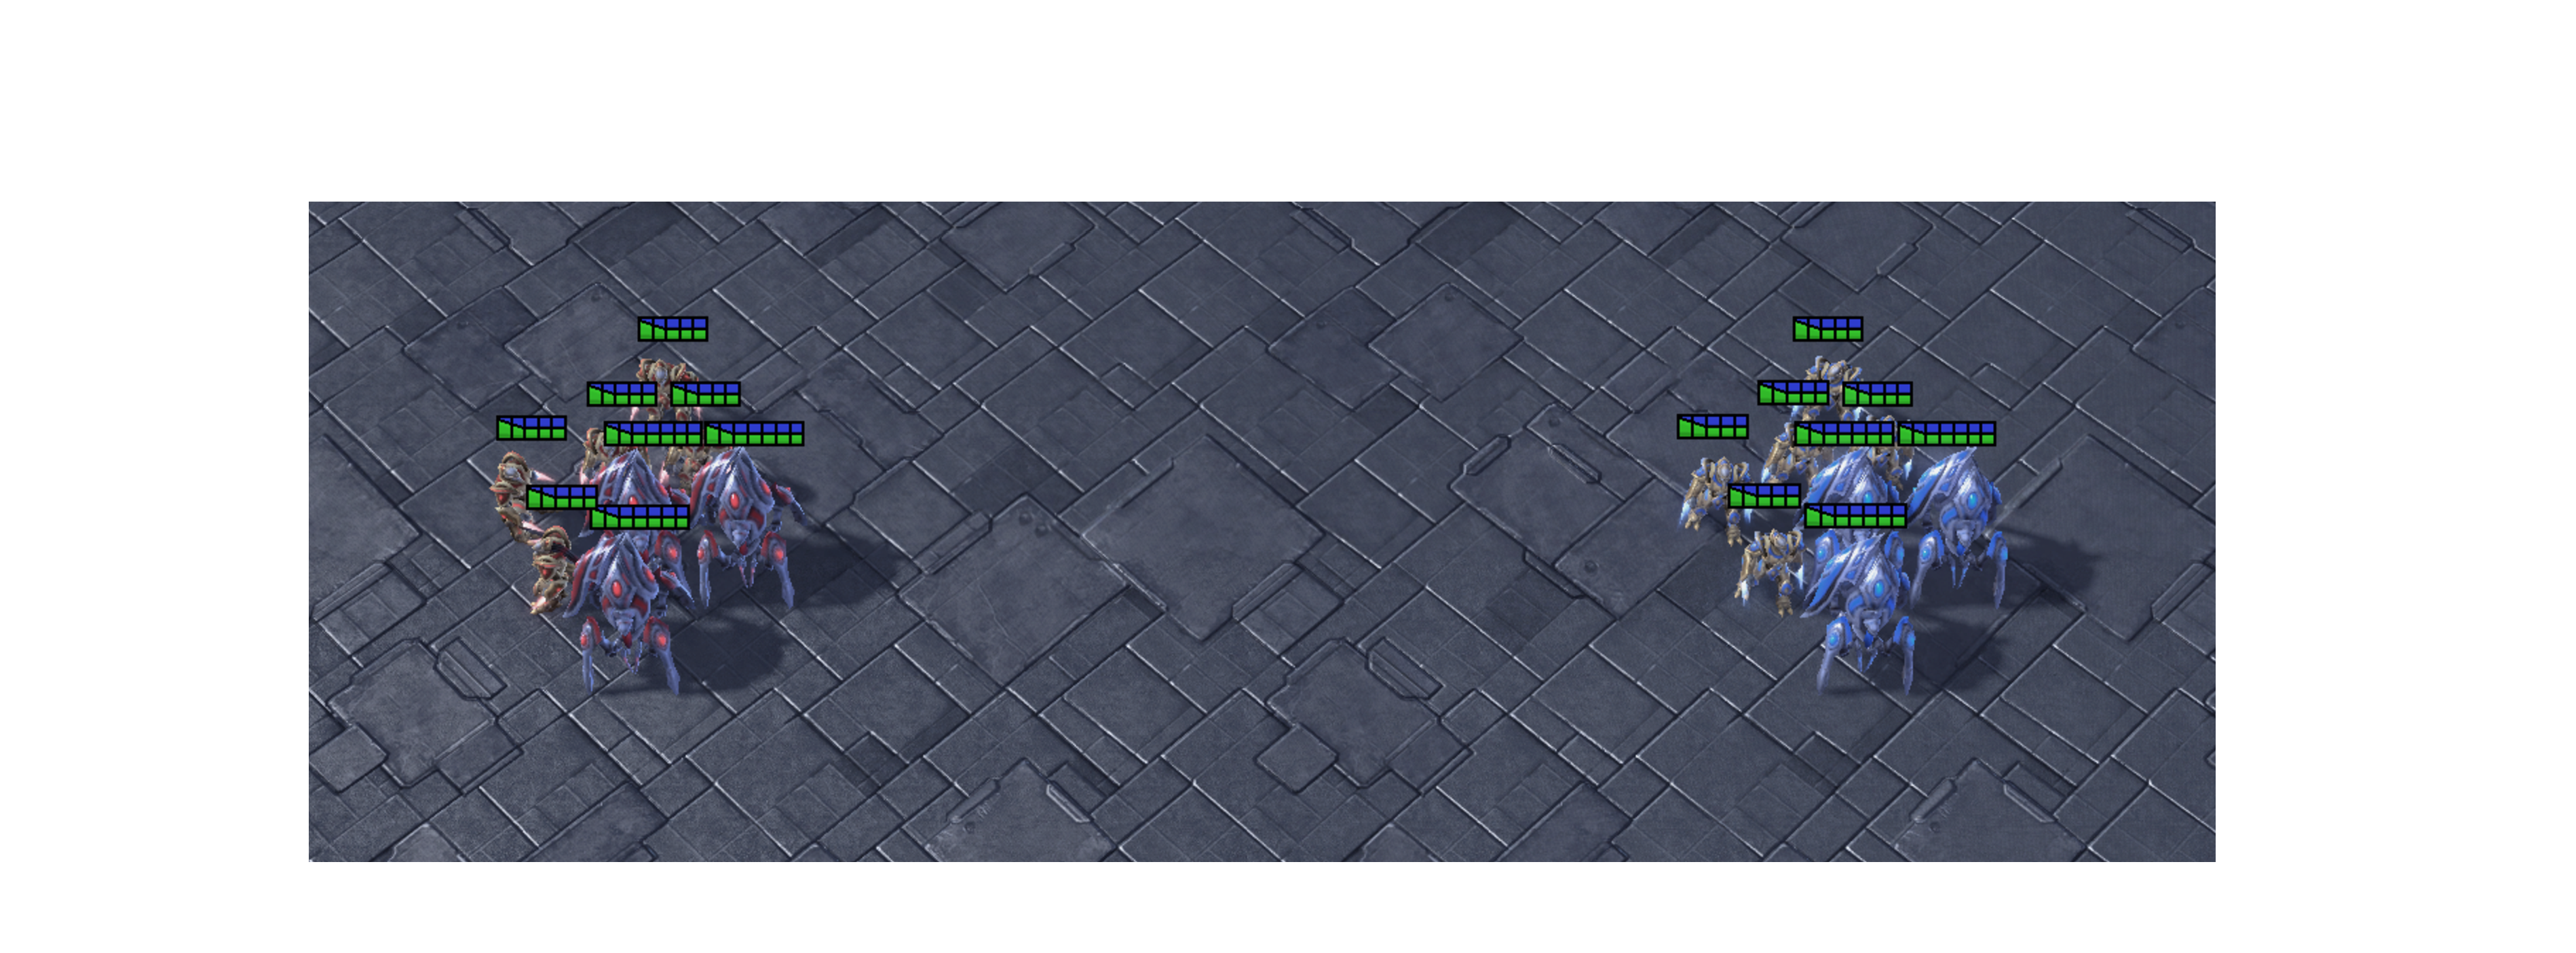
\includegraphics[height=2.3cm]{tex_thesis/figures/ch3/3s5z_screen.pdf}
         \caption{3s5z}
         \label{fig:ch3_3s5z}
     \end{subfigure}
    \caption{Two scenarios of the StarCraft multi-agent challenges.}
    \label{fig:ch3_smac}
\end{figure}

In SMAC, agents have partial observability defined by a sight range, a circle inside which they can observe allies and enemies.
There are different components in the observation.
An agent observes information about itself: its remaining hit points and shield points, its relative position with respect to the centre of the map and four Booleans representing the direction it can move in (NSWE). 
It also observes information about other agents within its sight range: the relative distance, relative x, relative y and the remaining hit points and shield points. 
If the other agent is an ally, it also observes its last performed action performed.
When the other agent is an enemy, it observes if this agent is within shooting range.
The shooting range is smaller than the sight range and depends on the unit type, and some units even attack in melee.

Within all scenarios, the agent has the choice of eight actions: do nothing, move in one of four directions (NSWE) or attack one of its three opponents.
Some actions are forbidden in SMAC, such as an attack if the opponent is not within shooting range.
Therefore, agents must consider which ones are available before choosing an action.

The state of the environment accumulates all information from agents' observations.
As described, an agent perceives other agents with distances relative to itself and does not know where it is on the map.
In the state, the agents' positions are encoded with their coordinates relative to the centre of the map.

At each timestep, the agent receives a zero or positive reward, common to each agent of the same team. 
This reward is a sum of three factors: a zero or positive reward for the damage dealt, a positive reward if an enemy unit's hit points reach zero, and a positive reward if all enemy units are defeated. 
Maximising the reward forces the team to neutralise every unit of the opposing team.

We hereafter describe both scenarios of Figure \ref{fig:ch3_smac}.
There are other types of units in other scenarios, and we refer the reader to \citep{samvelyan2019starcraft}.
In the $3m$ scenario, represented in Figure \ref{fig:ch3_3m}, six marines compete in two teams of three.
A marine has $45$ hit points and shoots at range, inflicting $6$ damage points to an opponent for each attack.
In the $3s5z$ scenario, represented in Figure \ref{fig:ch3_3s5z}, six stalkers and ten zealots compete in two teams of eight.
Both units have shield points in addition to hit points.
A shield receives a different amount of damage and regenerates over time if the unit is not attacked again for a given time.
A stalker has $80$ hit points and $80$ shield points.
It shoots at range, inflicting $13$ damage points to the shield, $12$ damage points to a zealot's hit points and $17$ to a stalker's hit points.
A zealot has 100 hits points and 50 shield points.
It attacks in melee and inflicts $16$ damage points to the shield and $14$ damage points to the hit points of a zealot or a stalker.

Finally, it can be intriguing to see an environment where two teams compete is considered cooperative.
This is because the built-in AI is stationary. 
These agents can be considered part of the environment and are not learning agents.
The built-in AI strategy can be described as rules-based.
Specifically, each agent moves toward the starting point of the opponent's team until it reaches the opposite side of the map and stops.
If they encounter opponents in their sight range, they select one as their target based on a priority score.
They will choose to attack the closest unit with the highest priority, which will remain the target until its priority drops or until it can no longer be attacked.
A unit's priority score is based on its type and current action.
For example, if two of the same units attack and the targeted unit stops attacking, its priority score will drop, and the built-in AI agents will select the other unit to attack.

\section{Value-based methods}
\label{sec:ch3_value}
\todo{check competition paper to add information}

Value-based methods aim to learn the optimal state-action value function $Q^{\pi^*}(s, u)$, such that the optimal policy is $\pi^*(s)=\argmax_{u} Q^{\pi^*}(s, u)$.
In SARL, one solution, called DQN \citep{Mnih2015}, is to approximate $Q$ with a neural network $\theta$ and learn $Q(s, u;\theta)$
by minimising the loss defined in Equation \ref{eq:ch2_dqnloss}.
More details are provided in Chapter \ref{ch:marl}.

As introduced in Section \ref{sec:ch3_intro}, there exist different modes of training and execution.
One possible centralised training and execution approach is to use DQN to train a centralised learner in a Dec-POMDP (\todo{MMDP boutiller}).
However, it is only possible if all agents can access the state $s$ during execution, resulting in the learning of $Q^{\boldsymbol{\pi}}(s,\mathbf{u}; \theta)$ by following the adapted DQN loss in Equation \ref{eq:ch3_centralQloss}.
\begin{equation}
\label{eq:ch3_centralQloss}
    \mathcal{L}(\theta) = \mathbb{E}_{\langle . \rangle\sim B} \big[\big(r_{t} + \gamma \max_{\mathbf{u}} Q(s_{t+1}, \mathbf{u}; \theta')- Q(s_{t}, \mathbf{\mathbf{u_t}}; \theta)\big)^{2}\big]
\end{equation}
Issues are that the joint action space scales exponentially with $n$, and in practice, agents select their action based only on their history of observation $(o, \tau)$ and not the state $s$.

For the second mode, the decentralised training and execution, each agent can learn its own Q-value independently $Q^{\pi^a}(o^a, u^a)$, agnostically of the existence of other agents.
IQL \citep{Tan1993} is the extension of Q-Learning (see Chapter \ref{ch:marl}).
The same with DQN has been performed \citep{TampuuDqnIQL}
One problem with IQL is that agents must select actions which maximise $Q(s_t, \mathbf{u_t})$ while ignoring, at any time, actions taken by other agents.

The third mode is centralised training with decentralised execution.
It is the one that interest us the most in this manuscript.
With CTDE methods, it is possible to approximate $Q(s_t, \mathbf{u_t})$ as a factorisation of individual $Q_a$ functions during training such that $\mathbf{u_t}$ maximises both the joint and the individual $Q_a$ functions.
To ensure this, individual $Q_a$ functions must satisfy the Individual-Global-Max condition (IGM)\citep{Son2019QTRAN:Learning} presented in Equation \ref{eq:ch3_igm}.

\begin{equation}
    \argmax_{\mathbf{u_t}} Q(s_t, \mathbf{u_t}) =\bigcup_{a}\argmax_{u_t^{a}} Q_{a}(s_t, u_t^{a})
    \label{eq:ch3_igm}
\end{equation}

Agents select actions based on their $Q_a$, now utility functions that factorise $Q_{tot}$ and not $Q$ function.

A solution proposed in QMIX \citep{Rashid2018} is to approximate $Q_{tot}$ as a function of all $Q_a$ and $s$ during training.


\subsection{QMIX} 
QMIX \citep{Rashid2018} is a CTDE method where the factorisation of $Q(s_t, \mathbf{u_t})$, denoted as $Q_{mix}(s_t, \mathbf{u_t})$, is performed as a function of the individual $Q_a$ functions and the state during training. It is defined in Equation \ref{eq:qmixappendix}.

\begin{equation}
     Q_{mix}=\text{Mixer} \left(Q_{a_1}(s_t, u_t^{a_1}) ,..,Q_{a_n}(s_t, u_t^{a_n}), s_t\right)
     \label{eq:qmixappendix}
\end{equation}

The mixer satisfies IGM by enforcing $\frac{\partial Q_{mix}(s_t, \mathbf{u_t})}{\partial Q_{a}(s_t, u_t^{a})} \geq 0 \text{ } \forall a \in \{a_1,..,a_n\}$ by constraining a hypernetwork \citep{Ha2016HyperNetworks} to produce positive weights in order to factorise $Q(s_t, \mathbf{u_t})$.
Formally, this is defined by a hypernetwork $h_p(.): \mathcal{S} \rightarrow \mathbb{R}^{|\phi|+}$ which takes the state $s_t$ as input and computes the strictly positive parameters\footnote{To be exact, the offsets defined by $h_p()$ are not constrained to be positive, only the weights.} $\phi$ of a main network $h_m(.)$.
This main network takes as input all individual $Q_a$ to compute $Q_{mix}$ with the positive weights and the offsets defined by $\phi$.
Together, $h_p(.)$ and $h_m(.)$ defines the mixer such that $h_m(.): \mathbb{R}^n \times \phi \rightarrow \mathbb{R}$ and $Q_{mix}(s_t, \mathbf{u_t}) = h_m\left(Q_{a_1}(),..,Q_{a_n}(), h_p(s_t)\right)$.
QMIX architecture is presented in Figure \ref{fig:qmix}.

The monotonicity of $Q_{mix}$ with respect to the individual $Q_a$ functions is satisfied because a neural network comprised of monotonic functions ($h_m$) and strictly positive weights ($h_p$) is monotonic with respect to its inputs ($Q_a$). 
Since we are in partial observability, individual $Q_a$ networks are RNNs made of GRU \citep{Chung2014EmpiricalModeling}.
The optimisation procedure follows the same principles of the DQN algorithm and the loss applied to $Q_{mix}(s_t, \mathbf{u_t})$ is defined in Equation \ref{eq:QMIX_loss}.

\begin{equation}
    \mathcal{L}(\theta) = \mathbb{E}_{\langle s_{t},\mathbf{u_{t}},r_{t},s_{t+1} \rangle \sim B}
    \bigg[  
    \big(r_{t} + \gamma \max_{\mathbf{u} \in \mathcal{U}} Q_{mix}(s_{t+1}, \mathbf{u}; \theta')
    - Q_{mix}(s_{t}, \mathbf{u_{t}}; \theta)\big)^{2}
    \bigg] 
    \label{eq:QMIX_loss}
\end{equation}

Since this method trains recurrent neural networks, the replay buffer does not store isolated transitions $\langle s_{t},\mathbf{u_{t}},r_{t},s_{t+1}\rangle$ but instead stores sequences of contiguous transitions.
Individual $Q_a$ networks are copied as well was as the mixer to produce target networks represented by $\theta'$.

In QMIX implementation, as in QVMix, individual $Q_a$ architecture follows the architecture presented in Figure \ref{fig:indivQ} and takes as input the previous action in addition to the observation.
Note that the hidden states of the recurrent neural network are represented by $h_t$ and their objective is to encode the agent's history $\tau_t$.



\begin{figure}[ht]
\centering

\begin{tikzpicture}[node distance=.5cm]

\tikzstyle{netbox} = [rectangle, rounded corners, minimum width=1cm, minimum height=1cm, draw=blue]
\tikzstyle{mixerbox} = [rectangle, rounded corners, minimum width=4.5cm, minimum height=1.5cm, draw=blue]
\tikzstyle{indixQbox} = [rectangle, rounded corners, minimum width=1.3cm, minimum height=2cm, draw=red, line width=1pt]
\tikzstyle{io} = [minimum width=0.2cm,minimum height=0.5cm]
\tikzstyle{emptynetbox} = [rectangle, rounded corners, minimum width=1cm, minimum height=1cm]

\node (output_node) [io] {$Q_{mix}^{tot}(s_t, \mathbf{u_t})$};
\node (mixerbox) [mixerbox, below=of output_node, yshift=-0cm, label={[xshift=-1.4cm, yshift=-1cm]Mixer}] {};
\node (indivQbox1) [indixQbox, below=of mixerbox, xshift=-1.2cm, yshift=-.5cm, label={[xshift=-0.22cm, yshift=.2cm]$Q_{a_1}(\tau^1_t, u^1_t)$}] {$Q_{a_1}$};
\node (indivQboxn) [indixQbox, below=of mixerbox, xshift=1.2cm, yshift=-.5cm, label={[xshift=0.22cm, yshift=.2cm]$Q_{a_n}(\tau^n_t, u^n_t)$}] {$Q_{a_n}$};
\node (mixer_net) [netbox, below=of output_node, yshift=-0.3cm] {$h_m$};
\node (param_net) [netbox, right=of mixer_net] {$h_p$};
\node (param_net2) [emptynetbox, left=of mixer_net] {};


\node (intput_node1) [io,below=of indivQbox1, yshift=-0cm, label={[xshift=1.2cm, yshift=1.2cm]. . .}] {$o^{a_1}_t$};
\node (intput_noden) [io,below=of indivQboxn, yshift=-0cm] {$o^{a_n}_t$};
\node (intput_nodestate) [io, right=of param_net] {$s_t$};
\node (intput_nodestate2) [io, left=of param_net2] {};

\draw [-Latex, thick] (intput_node1) -- (indivQbox1);
\draw [-Latex, thick] (intput_noden) -- (indivQboxn);
\draw [-Latex, thick] (indivQbox1) --  (mixer_net);
\draw [-Latex, thick] (indivQboxn) -- (mixer_net);
\draw [-Latex, thick] (param_net) -- (mixer_net) node[midway, yshift=0.3cm] {$|.|$};
\draw [-Latex, thick] (intput_nodestate) -- (param_net);
\draw [-Latex, thick] (mixer_net) -- (output_node);

%\draw[thick, rounded corners, draw=blue, fill=blue!50, opacity=0.2] ($(mixerbox.north west)+(-0.5,0.5)$) rectangle ($(indivQboxn.south east)+(1,-0.5)$);
\draw[thick, rounded corners, fill=red!50, opacity=0.2] ($(indivQbox1.north west)$) rectangle ($(indivQbox1.south east)$);
\draw[thick, rounded corners, fill=red!50, opacity=0.2] ($(indivQboxn.north west)$) rectangle ($(indivQboxn.south east)$);
\end{tikzpicture}
\caption{QMIX architecture. Individual $Q_a$ are represented in red and the mixing network is represented in blue.}
\label{fig:qmix}
\caption{Details of the QMIX and QVMix architecture.}
\end{figure}

\begin{figure}[t]
    \centering
\begin{tikzpicture}[node distance=.5cm]

\tikzstyle{netbox} = [rectangle, rounded corners, minimum width=2cm, minimum height=0.5cm,text centered, draw=red]
\tikzstyle{io} = [minimum width=0.2cm,minimum height=0.5cm, text centered]

\node (output_node) [io] {$\{Q_a(o_t^a, u^a_{j}) \forall u^a_j \in \mathcal{U}_a \}$};
\node (fctop) [netbox, below=of output_node, yshift=-0.3cm] {FC layer};
\node (rec_net) [netbox, below=of fctop, text width=2cm] {Recurrent layer};
\node (fcbot) [netbox, below=of rec_net] {FC layer};
\node (input_node) [io,below=of fcbot, yshift=-0.3cm] {$o^a_t$}%, u^a_{t-1}$};
\node (input_rec) [io,left=of rec_net, xshift=-0.3cm] {$h_{t-1}$};
\node (output_rec) [io,right=of rec_net, xshift=+0.3cm] {$h_t$};

\draw [-Latex, thick] (input_node) -- (fcbot);
\draw [-Latex, thick] (fcbot) -- (rec_net);
\draw [-Latex, thick] (rec_net) -- (fctop);
\draw [-Latex, thick] (fctop) -- (output_node);
\draw [-Latex, thick] (input_rec) -- (rec_net);
\draw [-Latex, thick] (rec_net) -- (output_rec);

\draw[thick, rounded corners, draw=red, fill=red!50, opacity=0.2] ($(fctop.north west)+(-0.5,0.5)$) rectangle ($(fcbot.south east)+(0.5,-0.5)$);
\draw[thick, rounded corners, draw=red] ($(fctop.north west)+(-0.5,0.5)$) rectangle ($(fcbot.south east)+(0.5,-0.5)$);
\end{tikzpicture}
\caption{Common individual $Q_a$ network implementation. The action space size defines the number of outputs of each agent network.}
\label{fig:indivQ}
\end{figure}

\subsection{MAVEN}
% to re write if time
Mahajan et. al. \cite{Mahajan2019MAVEN:Exploration} defined the class of state-joint-action value functions that cannot be represented by QMIX due to its monotonicity constraint.
They demonstrated the existence of payoff matrices in an n-player game with more than three actions per agent for which QMIX learns a suboptimal policy for any training duration, and for epsilon greedy and uniform exploration.
To tackle this problem, in the former QMIX architecture, they added a latent space that conditions individual $Q_a$ function networks with the objective of influencing agent behaviour.
This allows one to learn an ensemble of approximations and therefore an ensemble of policies to improve the exploration capabilities.
The latent variable is the input of a hypernetwork, such as $h_p$ in QMIX, that computes parameters for the fully connected layer linking recurrent cells to outputs in the individual $Q_a$ networks.
This latent variable $z$ is generated per episode and by a hierarchical policy network, taking as input the initial state of the environment together with a random variable (typically discrete and sampled from a uniform distribution).
The latent variable maps the different learnt strategies and the goal of the hierarchical policy network is to select the best strategy based on the initial state $s_0$ which is hypothetically known at testing.
The architecture of the individual $Q_a$ network of MAVEN is represented in Figure \ref{fig:maven}.

\begin{figure}[ht]
\centering
\begin{tikzpicture}[node distance=.5cm]

\tikzstyle{netbox} = [rectangle, rounded corners, minimum width=1.6cm, minimum height=0.7cm,text centered, draw=red]
\tikzstyle{netboxMaven} = [rectangle, rounded corners, minimum width=2cm, minimum height=0.7cm,text centered, draw=green]
\tikzstyle{io} = [text centered]

\node (output_node) [io] {$\{Q_a(s_t, u^a_{j}) \forall u^a_j \in \mathcal{U}_a \}$};
\node (fctop) [netbox, below=of output_node, yshift=-0.3cm] {FC layer};
\node (rec_net) [netbox, below=of fctop, text width=2cm] {Recurrent layer};
\node (fcbot) [netbox, below=of rec_net] {FC layer};
\node (intput_node) [io,below=of fcbot, yshift=-0cm] {$o^a_t, u^a_{t-1}$};
\node (input_rec) [io,left=of rec_net, xshift=-0.1cm] {$h_{t-1}$};
\node (output_rec) [io,right=of rec_net, xshift=+0.05cm] {$h_t$};

\draw [-Latex, thick] (intput_node) -- (fcbot);
\draw [-Latex, thick] (fcbot) -- (rec_net);
\draw [-Latex, thick] (rec_net) -- (fctop);
\draw [-Latex, thick] (fctop) -- (output_node);
\draw [-Latex, thick] (input_rec) -- (rec_net);
\draw [-Latex, thick] (rec_net) -- (output_rec);



\node (param_net) [netboxMaven, right=of fctop, xshift=1cm, text width=2.45cm] {Hypernetwork};
\node (latentvar) [io, right=of rec_net, xshift=.66cm, text width=2.5cm] {$z$};
\node (latent_net) [netboxMaven, right=of fcbot, xshift=1cm, text width=2.5cm] {Hierarchical policy network};
\node (intput_latent_1) [io,below=of latent_net, yshift=-0cm, xshift=-0.8cm] {$s_{t_0}$};
\node (intput_latent_2) [io,below=of latent_net, yshift=-0cm, xshift=0.8cm] {$x \sim P(x)$};
\draw [-Latex, thick] (param_net) -- (fctop);
\draw [-Latex, thick] (latentvar) -- (param_net);
\draw [-Latex, thick] (latent_net) -- (latentvar);
\draw [-Latex, thick] (intput_latent_1) -- (latent_net);
\draw [-Latex, thick] (intput_latent_2) -- (latent_net);


\draw[thick, rounded corners, draw=red, fill=red!50, opacity=0.2] ($(fctop.north)+(-1.5,0.3)$) rectangle ($(fcbot.south)+(1.5,-0.3)$);
%\draw[thick, rounded corners, draw=green, fill=green!80, opacity=0.2] ($(param_net.north)+(-1.5,0.3)$) rectangle ($(latent_net.south)+(1.5,-0.3)$);
\draw[thick, rounded corners, draw=red] ($(fctop.north)+(-1.5,0.3)$) rectangle ($(fcbot.south)+(1.5,-0.3)$);
\draw[thick, rounded corners, draw=green] ($(param_net.north)+(-1.5,0.3)$) rectangle ($(latent_net.south)+(1.5,-0.3)$);


\end{tikzpicture}
\caption{MAVEN modification of the individual $Q_a$ network.}
\label{fig:maven}

\caption{Details of the MAVEN architecture.}
\end{figure}

MAVEN's network objective function comprises three parts.
To optimise the two hypernetworks (the mixer and the latent space hypernetwork) and the individual recurrent neural networks, a part of the objective is the loss of QMIX defined in Equation \ref{eq:QMIX_loss}.
This loss is computed by fixing the hierarchical policy network and therefore the latent variable $z$.
To optimise the hierarchical policy network, any policy optimisation, such as policy gradient \citep{NIPS1999_464d828b}, computed with the total sum of rewards per episode can be used.
This second objective is computed by fixing both hypernetworks and the individual networks.
To ensure that different values of $z$ imply different behaviours, a mutual information loss between the latent variable and consecutive transitions is added as the third part of the objective.
This third part of the objective requires the introduction of a variational distribution and for further details on the MAVEN optimisation procedure and especially on the construction of the mutual information objective, we refer the reader to \cite{Mahajan2019MAVEN:Exploration}.



\subsection{QMIX}

In QMIX, the factorisation is achieved by a constrained hypernetwork \citep{Ha2016HyperNetworks} which links $s$ and $Q_a$ to $Q_{tot}$.
QVMix \citep{leroy2020qvmix} extends QMIX with the Deep Quality-Value method \citep{sabatelli2018deepQV,sabatelli2020deep}, learning both $V$ and $Q$, using the former as the target of the latter.
QPLEX \citep{wang2021qplex} extends QMIX with the dueling structure $Q = V + A$ \citep{wang2016dueling}, learning a factorisation of $V$ and $A$ with transformers \citep{vaswani2017attention}.
We selected these methods based on their IGM consistency, code availability, and results in the literature.

\subsection{MAVEN}
% to re write if time
Mahajan et. al. \cite{Mahajan2019MAVEN:Exploration} defined the class of state-joint-action value functions that cannot be represented by QMIX due to its monotonicity constraint.
They demonstrated the existence of payoff matrices in an n-player game with more than three actions per agent for which QMIX learns a suboptimal policy for any training duration, and for epsilon greedy and uniform exploration.
To tackle this problem, in the former QMIX architecture, they added a latent space that conditions individual $Q_a$ function networks with the objective of influencing agent behaviour.
This allows one to learn an ensemble of approximations and therefore an ensemble of policies to improve the exploration capabilities.
The latent variable is the input of a hypernetwork, such as $h_p$ in QMIX, that computes parameters for the fully connected layer linking recurrent cells to outputs in the individual $Q_a$ networks.
This latent variable $z$ is generated per episode and by a hierarchical policy network, taking as input the initial state of the environment together with a random variable (typically discrete and sampled from a uniform distribution).
The latent variable maps the different learnt strategies and the goal of the hierarchical policy network is to select the best strategy based on the initial state $s_0$ which is hypothetically known at testing.
The architecture of the individual $Q_a$ network of MAVEN is represented in Figure \ref{fig:maven}.

MAVEN's network objective function comprises three parts.
To optimise the two hypernetworks (the mixer and the latent space hypernetwork) and the individual recurrent neural networks, a part of the objective is the loss of QMIX defined in Equation \ref{eq:QMIX_loss}.
This loss is computed by fixing the hierarchical policy network and therefore the latent variable $z$.
To optimise the hierarchical policy network, any policy optimisation, such as policy gradient \citep{NIPS1999_464d828b}, computed with the total sum of rewards per episode can be used.
This second objective is computed by fixing both hypernetworks and the individual networks.
To ensure that different values of $z$ imply different behaviours, a mutual information loss between the latent variable and consecutive transitions is added as the third part of the objective.
This third part of the objective requires the introduction of a variational distribution and for further details on the MAVEN optimisation procedure and especially on the construction of the mutual information objective, we refer the reader to \cite{Mahajan2019MAVEN:Exploration}.

\subsection{QPLEX}

\subsection{Other methods}

\section{Policy-based methods}
\label{sec:ch3_policy}

\section{Related work}
\label{sec:ch3_rel_work}

Oroojlooy and Hajinezhad \citep{oroojlooy2022review} provide a review of cooperative MARL, including a more detailed list of applications.